\documentclass{article}
\usepackage[utf8]{inputenc}
\usepackage[hidelinks]{hyperref}
\usepackage{xcolor}
\usepackage[T1]{fontenc}
\usepackage{listings}
\usepackage{xcolor}
\usepackage{graphicx}
\usepackage[a4paper, left = 3cm, right = 3cm, top =2cm]{geometry}
\definecolor{codegreen}{rgb}{0,0.6,0}
\definecolor{codegray}{rgb}{0.5,0.5,0.5}
\definecolor{codepurple}{rgb}{0.58,0,0.82}
\definecolor{backcolour}{rgb}{0.95,0.95,0.92}
\definecolor{crimson}{HTML}{DC1420}
\definecolor{customGreen}{HTML}{228B22}
\definecolor{marron}{HTML}{804000}
\definecolor{orange}{HTML}{FFA500}
\lstdefinestyle{mystyle}{
    backgroundcolor=\color{backcolour},   
    commentstyle=\color{codegreen},
    keywordstyle=\color{magenta},
    numberstyle=\tiny\color{codegray},
    stringstyle=\color{codepurple},
    basicstyle=\ttfamily\footnotesize,
    breakatwhitespace=false,         
    breaklines=true,                 
    captionpos=b,                    
    keepspaces=true,                 
    numbers=left,                    
    numbersep=5pt,                  
    showspaces=false,                
    showstringspaces=false,
    showtabs=false,                  
    tabsize=2
}
\lstset{keepspaces=true, style=mystyle}

\title{\textcolor{crimson}{\Large{\textbf{Proyecto Final de Análisis Exploratorio de Datos}}} \\ \normalsize{\textit{Facultad de Matemática y Computación}} \\\normalsize{\textit{Ciencia de Datos \\ Grupo D111}}\\ \textcolor{customGreen}{\large{\textit{Dataset: Trees.}}}} 
\author{\textcolor{marron}{\normalsize{Guillermo Cepero García}} \\ \textcolor{marron}{\normalsize{Luis Ernesto Serras Rimada}} \\ \textcolor{marron}{\normalsize{Miguel Vadim Vilariño Pedraza}}}
\date{\today}
\begin{document}
\begin{titlepage}
    \begin{center}
    {
\includegraphics[width=0.15\textwidth]{img/matcom.jpg}\par}
    \vspace{0.1cm}
    {\bfseries\LARGE Ciencia de Datos \par}
    \vspace{0.2cm}
    {\scshape\Large  Facultad de Matamática y Computación\par}
    \vspace{0.6cm}
    {\scshape\Huge{\textcolor{crimson}{\textbf{Análisis Exploratorio de Datos \\ Proyecto Final}}} \par}
    \vspace{0.2cm}
    {\itshape\Large \textcolor{customGreen}{\large{\textit{Dataset: Trees.}}} \par}
    \vspace{0.8cm}
    {\large \textcolor{marron}{Integrantes:} \\ \normalsize{Guillermo Cepero García} \\ \normalsize{Luis Ernesto Serras Rimada} \\ \normalsize{Miguel Vadim Vilariño Pedraza} \par}
    \vspace{0.5cm}
    {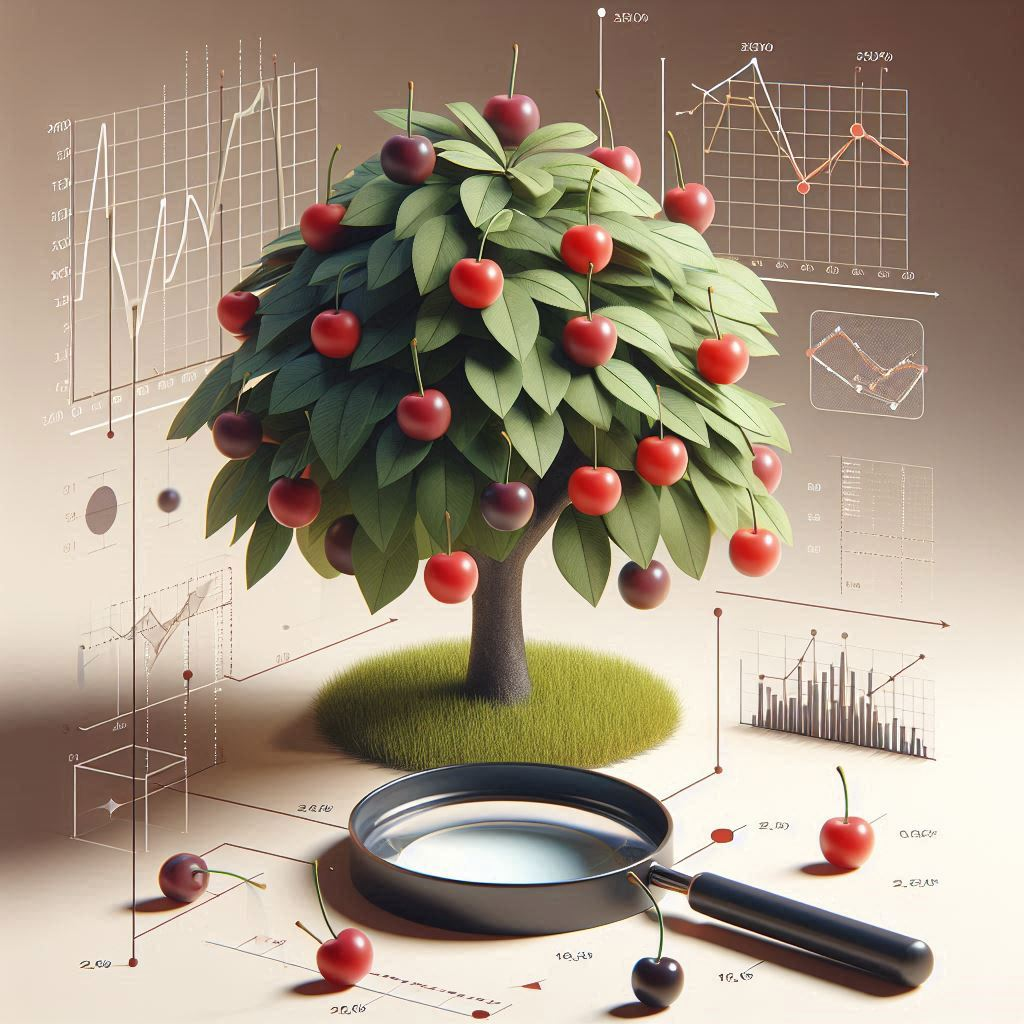
\includegraphics[width=0.85\textwidth]{img/cherry trees.jpeg}}
    \end{center}
\end{titlepage}
\newpage
\tableofcontents
\lstlistoflistings
\newpage
\section{Descripción de las variables}
\subsection{Presentación del dataset}
El dataset trees de \textcolor{blue}{RStudio} contiene información sobre la circunferencia (Girth), altura (Height) y volumen (Volume) de 31 árboles. Este análisis exploratorio de datos (EDA) tiene como objetivo examinar las variables del dataset, visualizar sus distribuciones y relaciones, y llegar a conclusiones basadas en los resultados obtenidos. El objetivo principal de este análisis es explorar las características de los árboles representados en el dataset, identificar patrones y relaciones entre las variables, y visualizar estos hallazgos de manera efectiva. Este análisis puede proporcionar información valiosa para estudios forestales, gestión de recursos naturales y aplicaciones en silvicultura.\\
A continuación, se presenta una muestra de los datos contenidos en el dataset:
\begin{lstlisting}[language=R, caption=Cargando y visualizando el dataset]
# Cargar el dataset
data(trees)

# Ver todas las filas del dataset
head(trees,31)

OUTPUT:
    Girth Height Volume
1    8.3     70   10.3
2    8.6     65   10.3
3    8.8     63   10.2
4   10.5     72   16.4
5   10.7     81   18.8
6   10.8     83   19.7
7   11.0     66   15.6
8   11.0     75   18.2
9   11.1     80   22.6
10  11.2     75   19.9
11  11.3     79   24.2
12  11.4     76   21.0
13  11.4     76   21.4
14  11.7     69   21.3
15  12.0     75   19.1
16  12.9     74   22.2
17  12.9     85   33.8
18  13.3     86   27.4
19  13.7     71   25.7
20  13.8     64   24.9
21  14.0     78   34.5
22  14.2     80   31.7
23  14.5     74   36.3
24  16.0     72   38.3
25  16.3     77   42.6
26  17.3     81   55.4
27  17.5     82   55.7
28  17.9     80   58.3
29  18.0     80   51.5
30  18.0     80   51.0
31  20.6     87   77.0
\end{lstlisting}

\newpage
\subsection{Análisis de las variables del dataset}
El dataset trees incluye las siguientes variables:\\
\emph{Girth:}
\begin{itemize}
    \item Descripción: Diámetro del tronco del árbol a 4.5 pies del suelo.
    \item Escala: Pulgadas.
    \item Tipo: Continua.
\end{itemize}
\emph{Height:}
\begin{itemize}
    \item Descripción: Altura del árbol.
    \item Escala: Pies.
    \item Tipo: Continua.
\end{itemize}
\emph{Volume:}
\begin{itemize}
    \item Descripción: Volumen de madera del árbol.
    \item Escala: Pies cúbicos.
    \item Tipo: Continua.
\end{itemize}
Para llevar a cabo este análisis, emplearemos diversas medidas estadísticas que nos proporcionarán una visión detallada de cada variable del dataset. Estas medidas incluyen la media, mediana, moda, varianza, desviación estándar, rango, valores máximo y mínimo, coeficiente de variación, simetría y curtosis.\\
A continuación, se presenta el código en \textcolor{blue}{R} que permite calcular estas medidas y se explican brevemente cada una de ellas.
\begin{lstlisting}[language=R, caption=Medidas]
# Cargar librerias necesarias
library(e1071)  
# Funcion para calcular medidas estadisticas
medidas <- function(x) {
c(Media = mean(x),# Media aritmetica
Mediana = median(x),# Valor central
Moda = as.numeric(names(sort(table(x), decreasing = TRUE)[1])),# Valor mas frecuente
Varianza = var(x),# Dispersion de los datos
Desviacion_Estandar = sd(x),# Raiz cuadrada de la varianza
Rango = diff(range(x)),# Diferencia entre el valor maximo y minimo
Maximo = max(x),# Valor maximo
Minimo = min(x),# Valor minimo
Coeficiente_Variacion = sd(x) / mean(x),# Relacion entre la desviacion estandar y la media
Simetria = skewness(x),# Medida de asimetria de la distribucion
Curtosis = kurtosis(x))}# Medida de la "altura" de la distribucion  
# Aplicar la funcion a cada variable del dataset trees
resultados <- sapply(trees, medidas)
# Mostrar resultados
print(resultados)
------------------------------------------------------------------------------------
OUTPUT:
                            Girth      Height      Volume
Media                    13.2483871 76.00000000  30.1709677
Mediana                  12.9000000 76.00000000  24.2000000
Moda                     11.0000000 80.00000000  10.3000000
Varianza                  9.8479140 40.60000000 270.2027957
Desviacion_Estandar       3.1381386  6.37181293  16.4378464
Rango                    12.3000000 24.00000000  66.8000000
Maximo                   20.6000000 87.00000000  77.0000000
Minimo                    8.3000000 63.00000000  10.2000000
Coeficiente_Variacion     0.2368695  0.08383964   0.5448233
Simetria                  0.5010559 -0.35687727   1.0132739
Curtosis                 -0.7109412 -0.72336766   0.2460393
\end{lstlisting}
\newpage
\subsubsection{Interpreteación de las medidas por variable}
Análisis por Variable:\\
\underline{Girth (Ancho)}:
\begin{itemize}
    \item Media: 13.2483871. Indica que el ancho promedio de los objetos medidos es aproximadamente 13.25 unidades.
    \item Mediana: 12.9. La mitad de los anchos son menores o iguales a 12.9, y la otra mitad son mayores o iguales a 12.9.
    \item Moda: 11. El valor más frecuentemente observado en el conjunto de datos es 11.
    \item Varianza: 9.8479140. Muestra la dispersión de los anchos alrededor de la media. Cuanto mayor sea el valor, mayor será la variabilidad.
    \item Desviación Estándar: 3.1381386. Indica la cantidad promedio que los anchos difieren de la media. Es la raíz cuadrada de la varianza.
    \item Rango: 12.3. La diferencia entre el valor máximo y mínimo observado en los anchos.
    \item Máximo: 20.6. El ancho más grande registrado.
    \item Mínimo: 8.3. El ancho más pequeño registrado.
    \item Coeficiente de Variación: 0.2368695. Expresa la desviación estándar como proporción de la media. Un valor bajo indica menos variabilidad.
    \item Simetría (Asimetría): 0.5010559. Indica la asimetría de la distribución. Valores positivos indican una distribución sesgada hacia la derecha, y negativos hacia la izquierda.
    \item Curtosis: -0.7109412. Mide la "altura" de la distribución. Valores negativos indican una cola pesada a la izquierda, lo que significa que los valores extremos son más probables de lo esperado en una distribución normal.
\end{itemize}
\underline{Height (Altura)}:
\begin{itemize}
    \item Media: 76. La altura promedio de los objetos es 76 unidades.
    \item Mediana: 76. La mitad de las alturas son menores o iguales a 76, y la otra mitad son mayores o iguales a 76.
    \item Moda: 80. El valor más frecuentemente observado en las alturas es 80.
    \item Varianza: 40.6. Indica la dispersión de las alturas alrededor de la media.
    \item Desviación Estándar: 6.37. Muestra la cantidad promedio que las alturas difieren de la media.
    \item Rango: 24. La diferencia entre el valor máximo y mínimo observado en las alturas.
    \item Máximo: 87. La altura más alta registrada.
    \item Mínimo: 63. La altura más baja registrada.
    \item Coeficiente de Variación: 0.08383964. Indica la variabilidad relativa de las alturas.
    \item Simetría (Asimetría): -0.357. Sugiere una leve asimetría hacia la izquierda.
    \item Curtosis: -0.723. Indica una cola pesada a la izquierda, similar a la observada en la Girth.
\end{itemize}
\underline{Volume (Volumen)}:
\begin{itemize}
    \item Media: 30.171. El volumen promedio de los objetos es aproximadamente 30.17 unidades cúbicas.
    \item Mediana: 24.2. La mitad de los volúmenes son menores o iguales a 24.2, y la otra mitad son mayores o iguales a 24.2.
    \item Moda: 10.3. El valor más frecuentemente observado en los volúmenes es 10.3.
    \item Varianza: 270.2. Muestra la dispersión de los volúmenes alrededor de la media.
    \item Desviación Estándar: 16.44. Indica la cantidad promedio que los volúmenes difieren de la media.
    \item Rango: 66.8. La diferencia entre el valor máximo y mínimo observado en los volúmenes.
    \item Máximo: 77. El volumen más grande registrado.
    \item Mínimo: 10.2. El volumen más pequeño registrado.
    \item Coeficiente de Variación: 0.5448233. Indica la variabilidad relativa de los volúmenes.
    \item Simetría (Asimetría): 1.013. Sugiere una distribución sesgada hacia la derecha.
    \item Curtosis: 0.246. Indica una distribución con colas más pesadas que una distribución normal, lo que sugiere una menor probabilidad de ocurrencia de valores extremos.
\end{itemize}
\textcolor{blue}{\emph{Observaciones}}:\\
Estas medidas estadísticas proporcionan una visión detallada de la distribución de las variables Girth, Height y Volume. Observamos variaciones significativas en la simetría y la curtosis entre las variables, lo que sugiere diferencias en la forma de sus distribuciones. Además, el coeficiente de variación(de Pearson para variables no ordinales) y la desviación estándar ofrecen insights sobre la variabilidad relativa y absoluta de cada variable, siendo particularmente útiles para comparar la consistencia de las medidas entre diferentes conjuntos de datos.
anomalías en los datos, facilitando así un análisis más profundo y detallado.\\ 
A continuación, se presentarán las visualizaciones correspondientes a cada variable y sus interrelaciones, proporcionando una visión clara y comprensible de la estructura del dataset.
\section{Visualización de los datos}
En esta sección, representaremos las variables y sus datos a través de diversas gráficas. Utilizaremos diferentes tipos de visualizaciones para explorar y entender mejor las relaciones entre las variables del dataset. Las gráficas nos permitirán identificar patrones, tendencias y posibles
\subsection{Histograma de distribución del volumen de los árboles}
Código en \textcolor{blue}{R}:
\begin{lstlisting}[language=R, caption=Histograma de distribución del volumen de los árboles]
library(ggplot2)
# Definir la funcion para formatear las etiquetas como enteros
format_enteros <- function(x) {
    round(x)
}
# Crear el histograma
ggplot(trees, aes(x = Volume)) +
    geom_histogram(binwidth = 5, fill = "skyblue", color = "black") +
    scale_y_continuous(labels = function(x) format_enteros(x)) + # Aplicar la funcion para formatear las etiquetas
    theme_classic() +
    labs(title = "Distribucion del Volumen de los arboles",
        x = "Volume (pies cubicos)",
        y = "Frecuencia")
\end{lstlisting}
\newpage
\textbf{OUTPUT}:
\begin{center} 
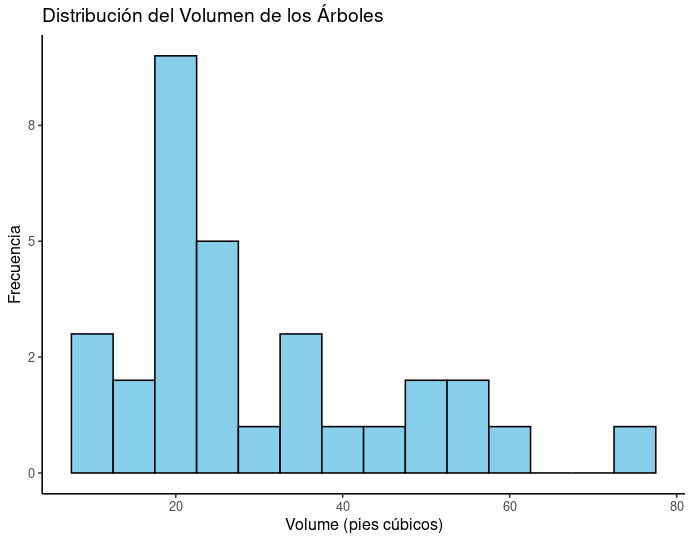
\includegraphics[width=1.0\textwidth]{code/Plots/histograma.png}
\end{center}
\large\textbf{\textcolor{cyan}{Interpretación:}}
\begin{itemize}
    \item \textbf{Eje X (Volumen en pies cúbicos)}: El eje X representa el volumen de los árboles medido en pies cúbicos. Los intervalos de volumen están divididos en rangos, como 0-10, 10-20, 20-30, etc.
    \item \textbf{Eje Y (Frecuencia)}: El eje Y muestra la frecuencia, es decir, el número de árboles que caen dentro de cada rango de volumen. En este aspecto se aplicó una función de redondeo para que se mostrasen las etiquetas como valores enteros.
    \item \textbf{Distribución}: La barra más alta se encuentra en el rango de 10-20 pies cúbicos, lo que indica que la mayoría de los árboles en este dataset tienen un volumen dentro de este rango.\\Las barras disminuyen en altura a medida que nos movemos hacia volúmenes mayores, sugiriendo que hay menos árboles con volúmenes muy grandes.
    \item \textbf{Tendencia Central}: La tendencia central del volumen de los árboles parece estar alrededor de 10-20 pies cúbicos, ya que este es el rango con la mayor frecuencia.
    \item \textbf{Variabilidad}: La variabilidad en los volúmenes de los árboles se puede observar en la dispersión de las barras a lo largo del eje X. Aunque la mayoría de los árboles tienen volúmenes entre 0 y 40 pies cúbicos, hay algunos que alcanzan hasta 80 pies cúbicos.
\end{itemize}
\subsection{BoxPlot de la altura de los árboles}
Después de analizar el histograma, procedemos a examinar el boxplot del dataset trees en \textcolor{blue}{RStudio}. Este boxplot nos proporciona una visión clara de la distribución de las alturas de los árboles en el dataset.\\
Código en \textcolor{blue}{R}:
\begin{lstlisting}[language=R, caption=BoxPlot de la altura de los árboles]
# Grafica de Boxplot
ggplot(trees, aes(x = "", y = Height)) +
    geom_boxplot(fill = "lightgreen", color = "darkgreen") +
    theme_light() +
    labs(title = "Boxplot de la Altura de los Arboles",
        x = "",
        y = "Height (altura en pies)")
\end{lstlisting}
\textbf{OUTPUT}:
\begin{center} 
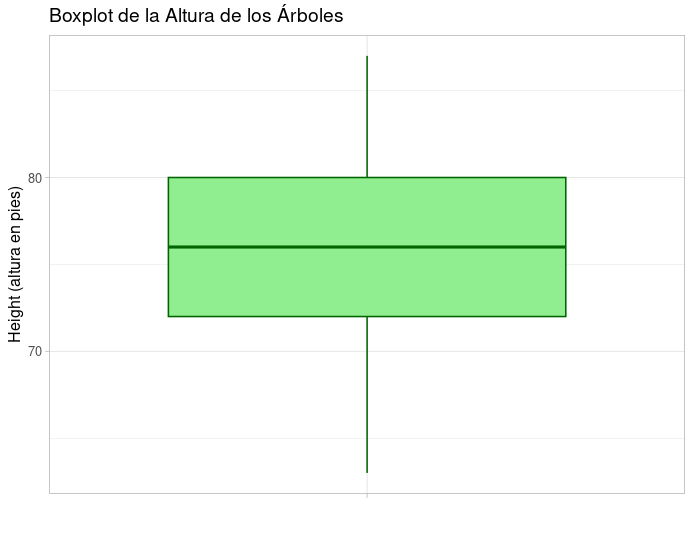
\includegraphics[width=0.8\textwidth]{code/Plots/BoxPlot.png}
\end{center}
El boxplot muestra la distribución de las alturas de los árboles, con los siguientes elementos clave:
\begin{itemize}
    \item \textbf{Línea Inferior del Bigote}: Representa el valor mínimo de la altura de los árboles, excluyendo cualquier valor atípico.
    \item \textbf{Borde Inferior de la Caja (Q1)}: Indica el primer cuartil, que es la mediana del primer 25% de los datos. En este caso, aproximadamente 70 pies.
    \item \textbf{Línea dentro de la Caja (Mediana o Q2)}: Marca la mediana de las alturas de los árboles, dividiendo el dataset en dos mitades iguales. Aquí, la mediana es alrededor de 75 pies.
    \item \textbf{Borde Superior de la Caja (Q3)}: Representa el tercer cuartil, que es la mediana del 75% superior de los datos. Aproximadamente 80 pies.
    \item \textbf{Línea Superior del Bigote}: Muestra el valor máximo de la altura de los árboles, excluyendo cualquier valor atípico.
    \item \textbf{Puntos Fuera de los Bigotes}: Estos puntos se consideran valores atípicos y representan alturas de árboles que son significativamente diferentes del resto de los datos.
\end{itemize}
\textbf{\textcolor{cyan}{Interpretación}}:
\begin{itemize}
    \item \textbf{Variabilidad}: La distancia entre el primer y tercer cuartil (Q1 y Q3) nos da una idea de la variabilidad de las alturas de los árboles. En este caso, la variabilidad es moderada.
    \item \textbf{Tendencia Central}: La mediana nos indica la altura central de los árboles en el dataset, que es aproximadamente 75 pies.
    \item \textbf{Valores Atípicos}: Cualquier punto fuera de los bigotes puede ser considerado un valor atípico, lo que sugiere que hay algunas alturas de árboles que son inusualmente altas o bajas en comparación con el resto del dataset.
\end{itemize}
\subsection{Gráfico de Barras de Girth}
Código en \textcolor{blue}{R}:
\begin{lstlisting}[language=R, caption=Gráfico d Barras d Girth]
# Grafico de barras para Girth
barplot(table(cut(trees$Girth, breaks = 5)),
        main = "Grafico de barras de Girth",
        xlab = "Intervalos de Girth",
        ylab = "Frecuencia",
        col = "lightblue",
        border = "black")
\end{lstlisting}
\textbf{OUTPUT}:
\begin{center} 
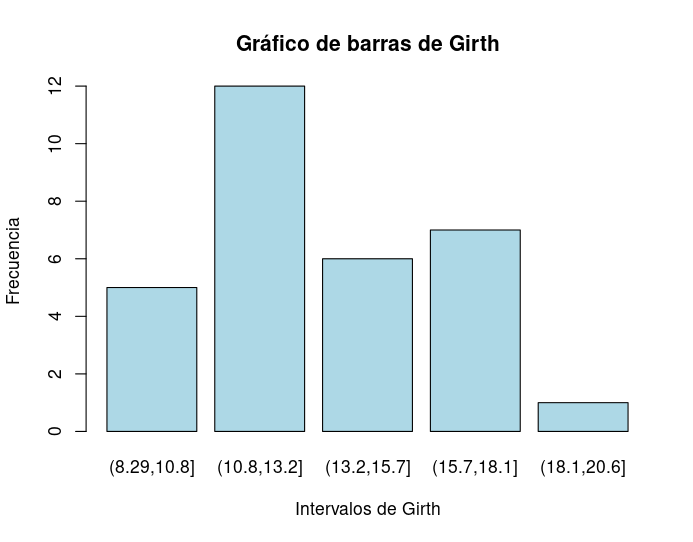
\includegraphics[width=1.0\textwidth]{code/Plots/Barra.png}
\end{center}
\large\textbf{\textcolor{cyan}{Interpretación:}}
\begin{itemize}
        \item \textbf{Intervalos de Girth}: El gráfico de barras muestra la frecuencia de los diámetros de los árboles (Girth) en diferentes intervalos. Esto nos permite ver cómo se distribuyen los diámetros en el dataset.
        \item \textbf{Frecuencia}: La altura de cada barra representa el número de árboles que caen dentro de cada intervalo de diámetro. Por ejemplo, si una barra es más alta, significa que hay más árboles con diámetros en ese rango específico.
        \item \textbf{Tendencias}: Observando el gráfico, podemos identificar si hay algún intervalo de diámetro que sea más común. Esto puede ser útil para entender las características predominantes de los árboles en el dataset.\\  \\Supongamos que el gráfico de barras muestra que la mayoría de los árboles tienen un diámetro (Girth) entre 10 y 15 unidades. Esto indicaría que los árboles en este dataset tienden a tener diámetros en ese rango, lo cual podría ser una característica importante a considerar en estudios forestales o de crecimiento de árboles. 
    \end{itemize}
\section{Relación entre las variables}
Después de analizar cada variable individualmente, ahora procederemos a explorar las relaciones entre las variables del dataset trees mediante el uso de gráficos. Esto nos permitirá identificar posibles correlaciones y patrones que podrían ser relevantes para nuestro estudio.
\subsection{Scatterplot de Relación entre Girth y Height}
El scatterplot titulado “Relación entre Girth y Height” muestra la relación entre la circunferencia (Girth) de los árboles en pulgadas y su altura (Height) en pies. Cada punto naranja en el gráfico representa un árbol del dataset.\\
Código en \textcolor{blue}{R}:
\begin{lstlisting}[language=R, caption=Scatterplot de Relación entre Girth y Height]
# Grafica de Scatter plot
ggplot(trees, aes(x = Girth, y = Height)) +
    geom_point(color = "darkorange", size = 3) +
    theme_minimal() +
    labs(title = "Relacion entre Girth y Height",
        x = "Girth (circunferencia en pulgadas)",
        y = "Height (altura en pies)")
\end{lstlisting}
\newpage
\textbf{\textbf{OUTPUT}:}
\begin{center} 
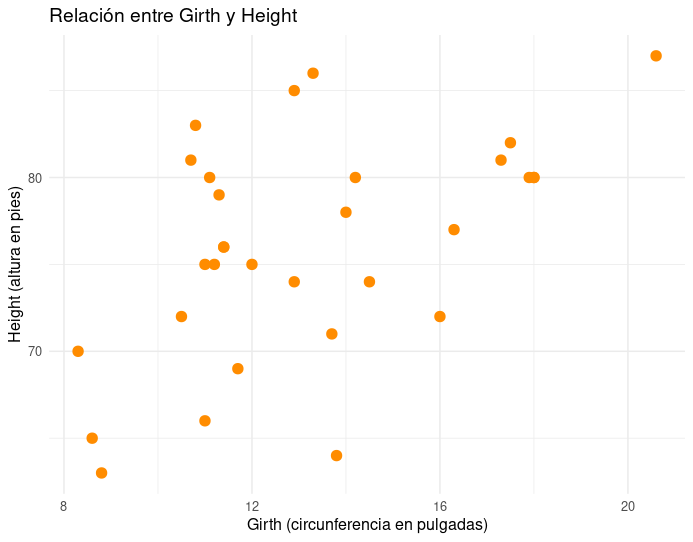
\includegraphics[width=1.0\textwidth]{code/Plots/scatter.png}
\end{center}
\large\textbf{\textcolor{cyan}{Interpretación:}}
\begin{itemize}
    \item \textbf{Eje Horizontal (Girth)}: Representa la circunferencia de los árboles en pulgadas, con un rango de 8 a 20 pulgadas.
    \item \textbf{Eje Vertical (Height)}: Indica la altura de los árboles en pies, con un rango de 60 a 80 pies.
    \item \textbf{Puntos de Datos}: Cada punto en el scatterplot muestra la relación entre la circunferencia y la altura de un árbol específico.
    \item \textbf{Relación Positiva }: Observamos una tendencia general donde, a medida que aumenta la circunferencia de los árboles, también tiende a aumentar su altura. Esto sugiere una relación positiva entre estas dos variables. \\ \\La tendencia positiva sugiere que, en general, los árboles con mayor circunferencia tienden a ser más altos. Sin embargo, la dispersión de los puntos también indica que hay variabilidad y posibles valores atípicos que merecen una investigación más detallada.
\end{itemize}
\newpage
\subsection{Relación entre Girth y Volume}
La gráfica presentada muestra la relación entre el perímetro (Girth) y el volumen (Volume) de un conjunto de árboles. En el eje horizontal se encuentra el perímetro, que varía de 8 a 20, mientras que en el eje vertical se encuentra el volumen, que varía de 10 a 70. Los puntos de datos en la gráfica indican una tendencia positiva, lo que sugiere que a medida que el perímetro de los árboles aumenta, el volumen también tiende a aumentar.\\
Código en \textcolor{blue}{R}:
\begin{lstlisting}[language=R, caption=Gráfico de Dispersión para la Relación entre Girth y Volume]
# Grafico de linea para Height y Volume
plot(trees$Height, trees$Volume,
        type = "l",
        main = "Relacion entre Height y Volume",
        xlab = "Height",
        ylab = "Volume",
        col = "red",
        lwd = 2)   
\end{lstlisting}
\textbf{\textbf{OUTPUT}:}
\begin{center} a observada en la gráfica sugiere que existe una proporción directa entre el perímetro y el volumen de los árboles. En términos prácticos, esto significa que al medir el perímetro de un árbol, se puede hacer una estimación razonable de su volumen. Este tipo de análisis es particularmente útil en la gestión forestal, donde se pueden utilizar mediciones del perímetro para estimar la cantidad de madera disponible sin necesidad de talar los árboles.
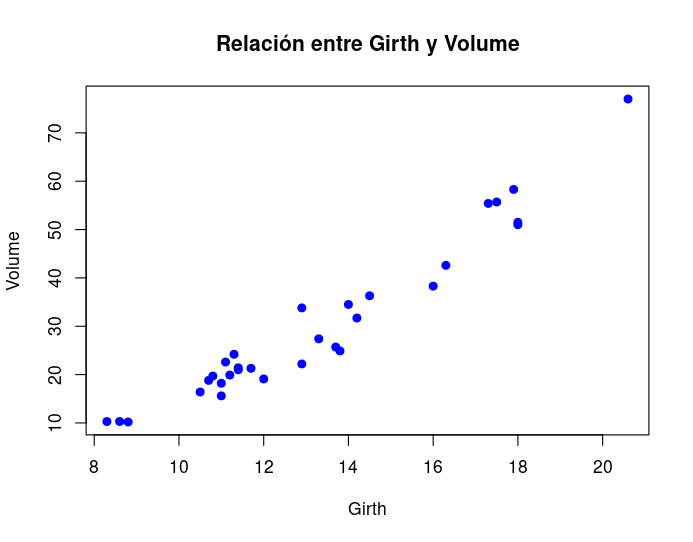
\includegraphics[width=1.0\textwidth]{code/Plots/dispersion.png}
\end{center}
\newpage
\large\textbf{\textcolor{cyan}{Interpretación:}}
\begin{itemize}
    \item \textbf{Tendencia Positiva}: La gráfica muestra una clara tendencia ascendente, lo que indica una correlación positiva entre el perímetro y el volumen. Esto significa que los árboles con mayor perímetro tienden a tener un mayor volumen.
    \item \textbf{Dispersión de Datos}: Aunque hay una tendencia general, los puntos de datos están dispersos, lo que sugiere que hay variabilidad en la relación entre el perímetro y el volumen. Esta dispersión puede deberse a otros factores que también influyen en el volumen de los árboles, como la especie, la edad, y las condiciones ambientales.
    \item \textbf{Concenctración de Datos}:  La mayoría de los puntos de datos se concentran en los valores inferiores del gráfico, con un esparcimiento mayor a medida que ambos valores aumentan. Esto podría indicar que la mayoría de los árboles en el conjunto de datos tienen perímetros y volúmenes más pequeños.
    \end{itemize}
La relación positiva observada en la gráfica sugiere que existe una proporción directa entre el perímetro y el volumen de los árboles. En términos prácticos, esto significa que al medir el perímetro de un árbol, se puede hacer una estimación razonable de su volumen. Este tipo de análisis es particularmente útil en la gestión forestal, donde se pueden utilizar mediciones del perímetro para estimar la cantidad de madera disponible sin necesidad de talar los árboles.
\subsection{Matriz de Correlación}
Por último, pasemos a la matriz de correlación. Esta matriz es una tabla que muestra los coeficientes de correlación entre múltiples variables. Cada celda en la matriz indica la correlación entre dos variables específicas, con valores que oscilan entre -1 y 1. Un valor de 1 indica una correlación positiva perfecta, -1 indica una correlación negativa perfecta, y 0 indica que no hay correlación entre las variables:\\
Código en \textcolor{blue}{R}:
\begin{lstlisting}[language=R, caption=Matriz de Correlación]
# Matriz de correlacion
cor(trees)

# Cargar librerias necesarias
library(ggplot2)
library(reshape2)

# Calcular la matriz de correlacion
cor_matrix <- cor(trees)

# Mostrar la matriz de correlacion
print(cor_matrix)

OUTPUT:

           Girth    Height    Volume
Girth  1.0000000 0.5192801 0.9678377
Height 0.5192801 1.0000000 0.6001130
Volume 0.9678377 0.6001130 1.0000000
\end{lstlisting}
Luego, se convierte en un formato adecuado para gráficos, y se utiliza \textbf{ggplot2} para visualizar esta matriz como un \textbf{gráfico de mosaico}, donde la intensidad del color indica el grado de correlación entre las variables de la siguiente forma:
\newpage
Código en \textcolor{blue}{R}:
\begin{lstlisting}[language=R, caption=Gráfica de Mosaico para la Matriz de Correlación]
# Convertir la matriz de correlacion en un formato largo
cor_data <- melt(cor_matrix)
    
# Crear la grafica de la matriz de correlacion
ggplot(data = cor_data, aes(x = Var1, y = Var2, fill = value)) +
    geom_tile() +
    scale_fill_gradient2(low = "blue", high = "red", mid = "white", 
                        midpoint = 0, limit = c(-1, 1), space = "Lab", 
                        name="Correlacion") +
    theme_minimal() +
    theme(axis.text.x = element_text(angle = 45, vjust = 1, 
                                    size = 12, hjust = 1)) +
    coord_fixed() +
    labs(title = "Matriz de Correlacion del Dataset Trees",
        x = "Variables",
        y = "Variables")
\end{lstlisting}
\textbf{\textbf{OUTPUT}:}
\begin{center} 
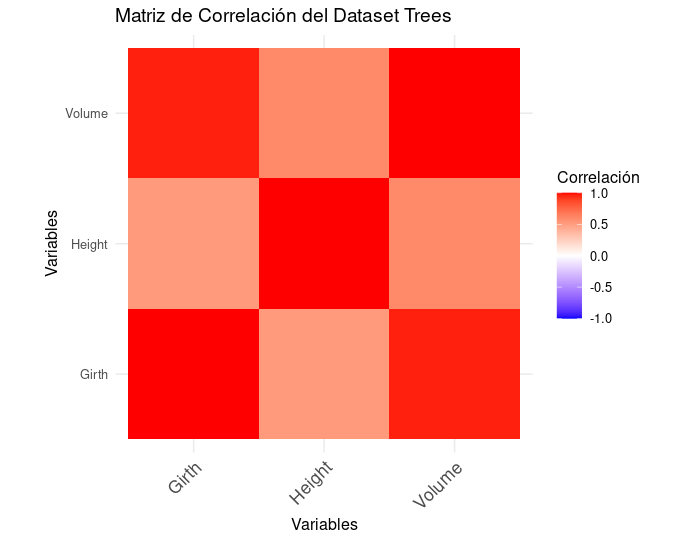
\includegraphics[width=0.7\textwidth]{code/Plots/Matriz de correlacion.png}
\end{center}
\emph{\textcolor{blue}{Observaciones:}}
\begin{itemize}
    \item \textbf{melt()} de \textit{reshape2} convierte la matriz de correlación en un formato de datos largo \textbf{(long format)}. Esto es necesario porque \textit{ggplot2} trabaja mejor con datos en formato largo o ancho \textbf{(wide format)} para ciertos tipos de gráficos.
    \item \textbf{geom\_tile()}: Crea un gráfico de mosaico \textbf{(tile plot)} donde cada celda representa la correlación entre dos variables.
    \item \textbf{scale\_fill\_gradient2()}: Define cómo se deben colorear las celdas basándose en su valor de correlación. En este caso, los valores negativos se muestran en azul, los positivos en rojo, y los cercanos a cero en blanco.
    \item \textbf{theme\_minimal()}: Aplica un tema minimalista al gráfico.
    \item \textbf{coord\_fixed()}: Asegura que las unidades de medida sean consistentes en ambos ejes.
    \item \textbf{labs()}: Define títulos y etiquetas para los ejes y el gráfico completo.
\end{itemize}
En resumen, estos códigos calculan la matriz de correlación de un conjunto de datos, la convierte en un formato adecuado para gráficos, y luego utiliza ggplot2 para visualizar esta matriz como un gráfico de mosaico, donde la intensidad del color indica el grado de correlación entre las variables.

Diagonal Principal (Girth, Height, Volume):
\begin{itemize}
    \item Girth vs Girth: 1.0000000
    \item Height vs Height: 1.0000000
    \item Volume vs Volume: 1.0000000
\end{itemize}
Estos valores son todos 1, lo que significa que cada característica tiene una correlación perfecta consigo misma. Es decir, un árbol grande (alto giro) será siempre grande (alto volumen) y viceversa, ya que estamos hablando de la misma característica medida en diferentes formas.\\
\large\textbf{\textcolor{cyan}{Interpretación:}}\\
\textbf{\underline{Relaciones entre Pares de Variables:}}
\begin{itemize}
    \item Girth vs Height: 0.5192801 \\ Esta correlación indica que hay una relación positiva moderada entre el giro y la altura de los árboles. Esto significa que los árboles más grandes tienden a ser también más altos, pero no hay una correlación perfecta, lo que sugiere que hay otros factores involucrados además del tamaño del tronco.
    \item Height vs Volume: 0.6001130 \\ Esta correlación muestra una relación positiva débil a moderada entre la altura y el volumen. Aunque existe una tendencia de que los árboles más altos tengan mayor volumen, el coeficiente es relativamente bajo, lo que indica que hay otras características importantes que influyen en el volumen del árbol además de su altura.
    \item Girth vs Volume: 0.9678377 \\ Este valor alto de correlación (cerca de 0.97) indica una fuerte relación positiva entre el giro y el volumen. Esto sugiere que los árboles con un giro más grande tienden a tener un volumen interior más grande, lo cual es esperable dado que el giro es una medida del diámetro del tronco, que directamente afecta el volumen interior del árbol.
\end{itemize}
En general, la matriz de correlación revela que hay una fuerte relación entre el giro y el volumen, lo que es intuitivo ya que el giro (diámetro del tronco) influirá directamente en el volumen interior del árbol. Sin embargo, la relación entre la altura y el volumen es menos fuerte, lo que sugiere que aunque haya una tendencia general de que los árboles más altos tengan mayor volumen, hay otros factores (como la densidad del árbol) que también juegan un papel importante. La correlación entre el giro y la altura es moderada, lo que indica que aunque hay una relación, existen otros factores que también contribuyen significativamente a la altura de un árbol.
\newpage
\section{Conclusiones}
El presente proyecto se centra en un análisis detallado del conjunto de datos "trees", enfocado en variables clave como la altura, el diámetro y el volumen de los árboles. Mediante el uso de técnicas avanzadas de Análisis Exploratorio de Datos (EDA), hemos logrado profundizar en la comprensión de la estructura interna y las relaciones existentes entre las variables del dataset.\\ \\ 
Los resultados obtenidos a través de nuestro estudio revelan patrones estadísticamente significativos que han permitido el desarrollo de modelos predictivos robustos, capaces de predecir con notable precisión el volumen de los árboles basándose en sus características físicas. Esta capacidad de predicción no solo representa un avance significativo en el entendimiento de los factores que influyen en el volumen arbóreo, sino que también abre nuevas posibilidades para su aplicación práctica.\\ \\
En resumen, el análisis exploratorio de datos realizado sobre el conjunto "trees" ha demostrado ser una herramienta poderosa para descubrir relaciones ocultas y generar conocimientos útiles. La aplicación de estos hallazgos tiene el potencial de transformar la forma en que se abordan las cuestiones relacionadas con la conservación y gestión de los recursos forestales, marcando un hito en la investigación y práctica ambiental.
\clearpage
\section{Metodología}
\begin{enumerate}
    \item \textbf{\textcolor{blue}{Recopilación de Datos: }}\\ Nuestro primer paso fue recopilar información relevante para el análisis de nuestro proyecto. Para ello, nos apoyamos en dos fuentes principales: los contenidos impartidos en las conferencias y clases prácticas de la asignatura y el libro de texto recomenadado. Los contenidos de clases proporcionaron una visión actualizada y detallada de los temas tratados, mientras que el libro de texto sirvió como referencia fundamental para entender los conceptos básicos y avanzados necesarios para nuestra investigación. También nos apoyamos de la documentación oficial de todos los formatos de tipografía y programación que utilizamos. \\ Las imágenes utilizadas (exceptuando el logo de MatCom) fueron generadas por una IA:\\ 
\url{https://copilot.microsoft.com/images/create?}
    \item \textbf{\textcolor{blue}{Herramientas de Desarrollo: }}\\ Para la obtención del dataset \textbf{\textcolor{customGreen}{Trees}}, el desarrollo y análisis de nuestro proyecto, optamos por utilizar \textcolor{blue}{RStudio}, una plataforma integrada para el lenguaje de programación \textcolor{blue}{R}. \textcolor{blue}{RStudio} facilita la escritura de código, la visualización de datos y la creación de informes, lo cual resultó esencial para nuestro trabajo. Además, empleamos \textcolor{gray}{RMarkdown}, una herramienta que permite combinar código \textcolor{blue}{R}, texto narrativo y elementos gráficos en un único documento. Esto no solo agiliza la generación de informes y presentaciones, sino que también asegura la reproducibilidad de nuestros análisis.
    \item \textbf{\textcolor{blue}{Proceso Analítico: }}\\ El proceso analítico comenzó con la preparación y estudio de los datos recopilados. Utilizando \textcolor{blue}{RStudio}, donde aplicamos diversas técnicas estadísticas para explorar las relaciones entre las variables para identificar patrones y analizar su comportamiento de forma satisfactoria.
    \item \textbf{\textcolor{blue}{Generación del Informe: }}\\ Para documentar nuestros hallazgos y procesos, recurrimos a \textcolor{gray}{LaTeX}, una herramienta de tipografía que permite crear documentos profesionales con un alto nivel de personalización. De esta forma pudimos generar un informe coherente y bien estructurado que incluye tanto el análisis estadístico como la interpretación de los resultados y unas conclusiones finales.
    \item \textbf{\textcolor{blue}{Generación de  la Presentación: }}\\ Finalmente, en interés de desarrollar un recurso para la exposición desarrollamos una presentacion utilizando el entorno de \textcolor{blue}{RStudio} con la herrrmienta de \textcolor{gray}{RMarkdown} para generar presentaciones en formato ioslide de \textcolor{orange}{HTML} de forma resumida, utilizando además un documento de estilo en formato \textcolor{green}{CSS (style.css)} para darle una ambientación innovadora y atractiva a la presentación.
\end{enumerate}

\cleardoublepage
\begin{titlepage}
    \begin{center}
    {\scshape\Huge{\textcolor{crimson}{\textbf{Fin}}} \par}
    \vspace{0.4cm}
    {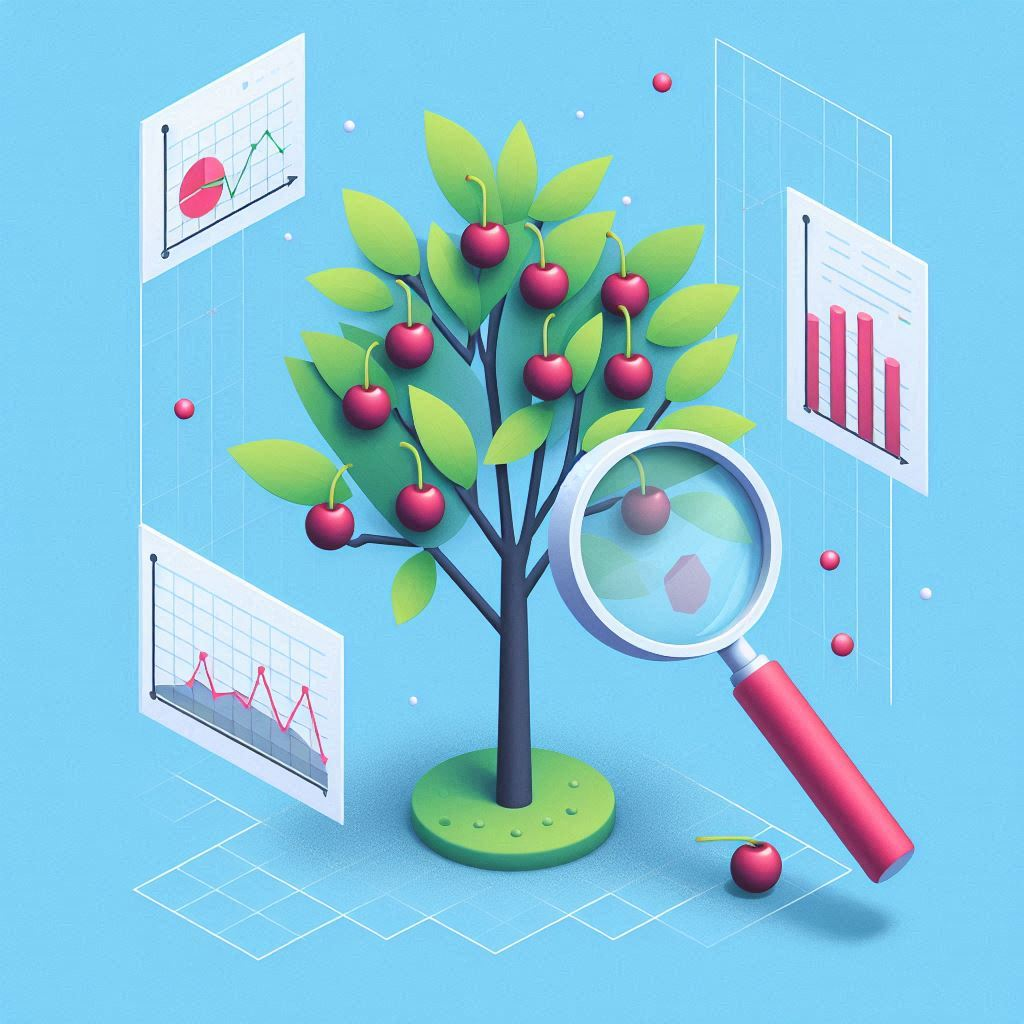
\includegraphics[width=1.0\textwidth]{img/cherrytrees2.jpeg}}
    \vspace{0.1cm}
    {\itshape\Large \textcolor{customGreen}{\large{\textit{Muchas gracias por su atención.\\Esperamos que nuestro proyecto haya sido de su agrado.}}} \par}
    \end{center}
\end{titlepage}
\end{document}
